\begin{center}
    \begin{figure}[H]
        \centering

        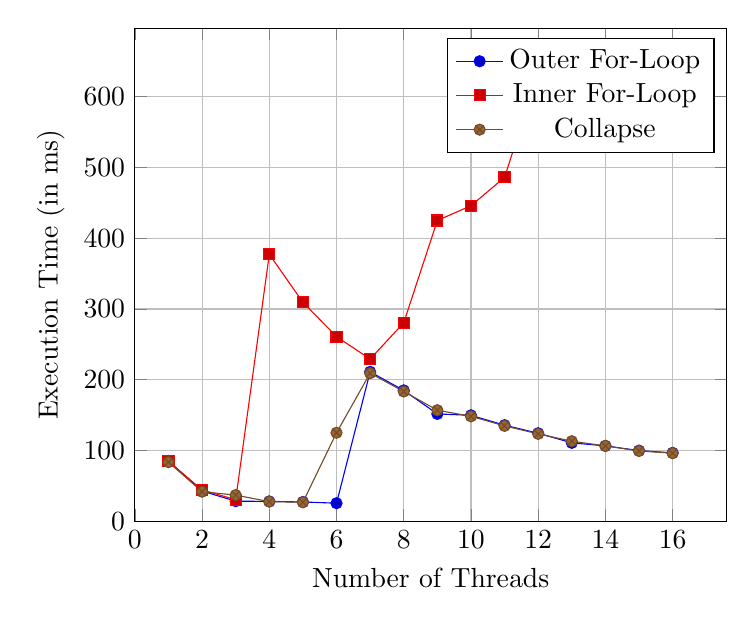
\begin{tikzpicture}
            \begin{axis}[
                title={},
                width=0.75\textwidth,
                xlabel={Number of Threads},
                ylabel={Execution Time (in ms)},
                xmin=0,
                ymin=0,
                grid=major
            ]
                \addplot coordinates {
                    (1,85.2391)(2,42.7317)(3,28.4423)(4,28.1247)(5,27.335)(6,25.593)(7,211.165)(8,185.023)(9,151.782)(10,149.757)(11,135.83)(12,124.469)(13,110.867)(14,106.599)(15,99.9)(16,96.7411)
                };
                \addlegendentry{Outer For-Loop}

                \addplot coordinates {
                    (1,84.644)(2,44.4306)(3,30.42)(4,377.29)(5,309.466)(6,261.024)(7,229.236)(8,280.602)(9,425.051)(10,445.941)(11,486.054)(12,633.441)(13,535.267)(14,607.319)(15,581.959)(16,578.969)
                };
                \addlegendentry{Inner For-Loop}       

                \addplot coordinates {
                    (1,83.6025)(2,41.8485)(3,37.0192)(4,27.7715)(5,26.8852)(6,125.15)(7,209.314)(8,183.416)(9,157)(10,148.357)(11,134.859)(12,123.538)(13,113.176)(14,106.568)(15,99.4303)(16,96.253)
                };
                \addlegendentry{Collapse}
            \end{axis}
        \end{tikzpicture}
        \caption{Grayscale Performance Tests dice\_large.png}
    \end{figure}
\end{center}